\documentclass[../ImageClassifier.tex]{subfiles}

\begin{document}
    Before we can start with training, we need to create the dataset from the previously downloaded and edited images.
    The number of images per keyword after the previous is normally around 600.
    Now the images are splitted into a testing set (80\%) and a validation set (20\%).
    With a smaller amount of images per keyword, like in this project, there is a high risk for overfitting.
    A way to prevent this, is to augment the small number of images in and only in the test dataset with zooming, rotation, width shift range, height shift range, shear range and horizontal flip.
    \begin{figure}[H]
        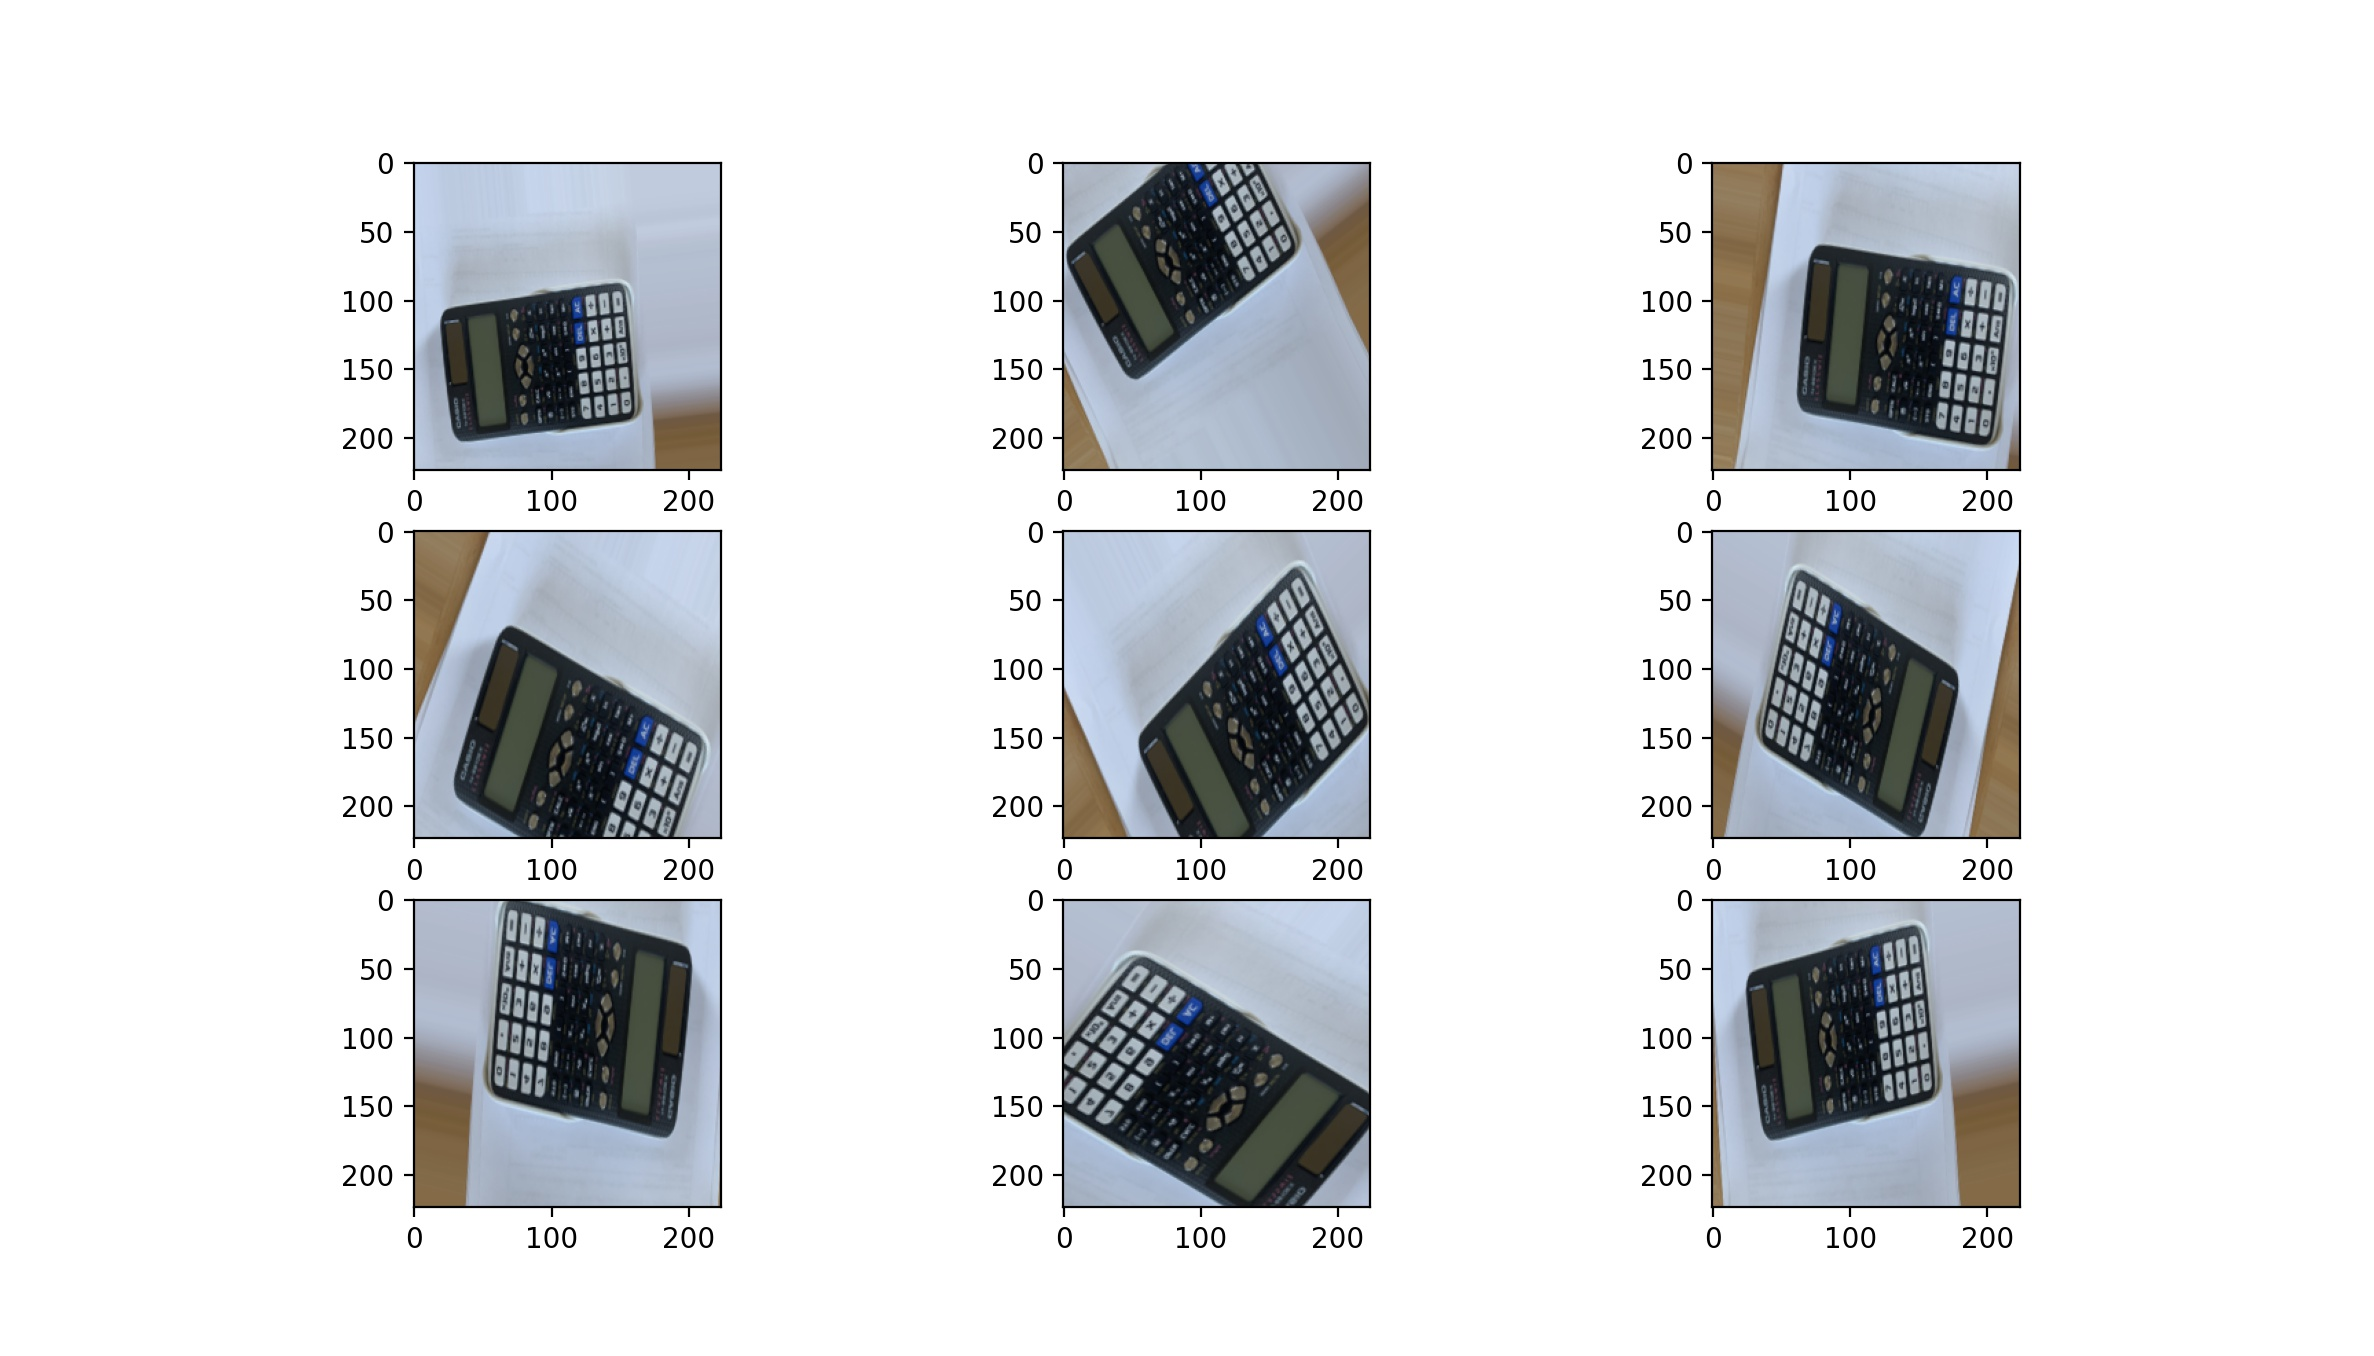
\includegraphics[width=\textwidth,height=\textheight,keepaspectratio]{./attachments/augmentation/augmentation.jpg}
        \caption{Image augmentation}
        \label{fig:image augmentation}
    \end{figure}
\end{document}
